\documentclass[a4paper,10pt]{article}
\usepackage[utf8]{inputenc}
\usepackage{frontespizio}
\usepackage{listings}
\usepackage{pdfpages}
\usepackage[usenames,dvipsnames]{color}
\usepackage{hyperref}

\definecolor{codegreen}{rgb}{0,0.6,0}
\definecolor{codegray}{rgb}{0.5,0.5,0.5}
\definecolor{codepurple}{rgb}{0.58,0,0.82}
\definecolor{backcolour}{rgb}{0.95,0.95,0.92}

\lstdefinestyle{mystyle}{
    backgroundcolor=\color{backcolour},   
    commentstyle=\color{codegreen},
    keywordstyle=\color{magenta},
    numberstyle=\tiny\color{codegray},
    stringstyle=\color{codepurple},
    basicstyle=\footnotesize,
    breakatwhitespace=false,         
    breaklines=true,                 
    captionpos=b,                    
    keepspaces=true,                 
    numbers=left,                    
    numbersep=5pt,                  
    showspaces=false,                
    showstringspaces=false,
    showtabs=false,                  
    tabsize=2
}
\lstset{style=mystyle}

% Title Page
\title{Relazione progetto di Basi di Dati}
\author{Giovanni Liboni}


\begin{document}
\begin{frontespizio}

\Universita{Verona}
\Dipartimento{Informatica}
\Corso[Laurea]{Informatica}
\Titoletto{Consegna G4 - Sistema informativo per la gestione dell'emissione di biglietti aerei}
\Titolo{Relazione finale del progetto di Basi di Dati }

\Candidato[VR363021]{Giovanni Liboni}

\Annoaccademico{2013-2014}
\end{frontespizio}

\tableofcontents

\newpage

\part{Progetto della basi di dati}

\section{Progetto concettuale}
Qui di seguito si riporta il diagramma Entit\`a - Relazione e lo schema concettuale ricavati dalle specifiche del progetto.
A partire da questo schema si sono scritte le tabelle per la Base di Dati.

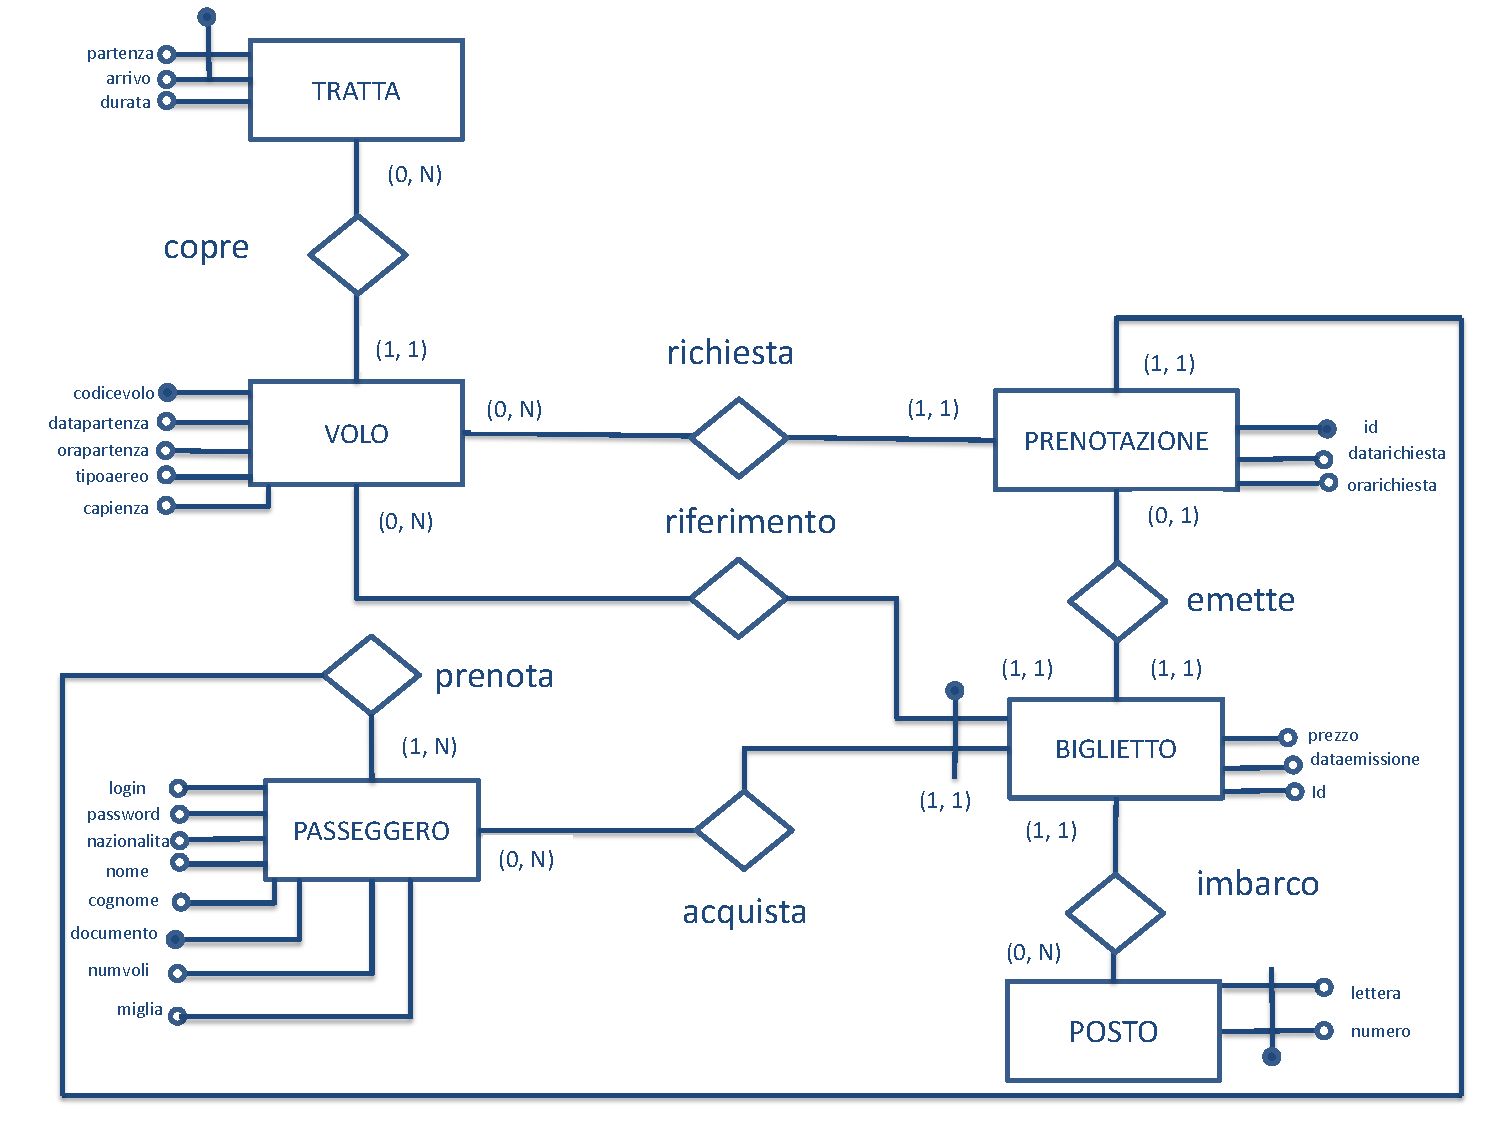
\includegraphics[scale=0.5]{er.pdf}

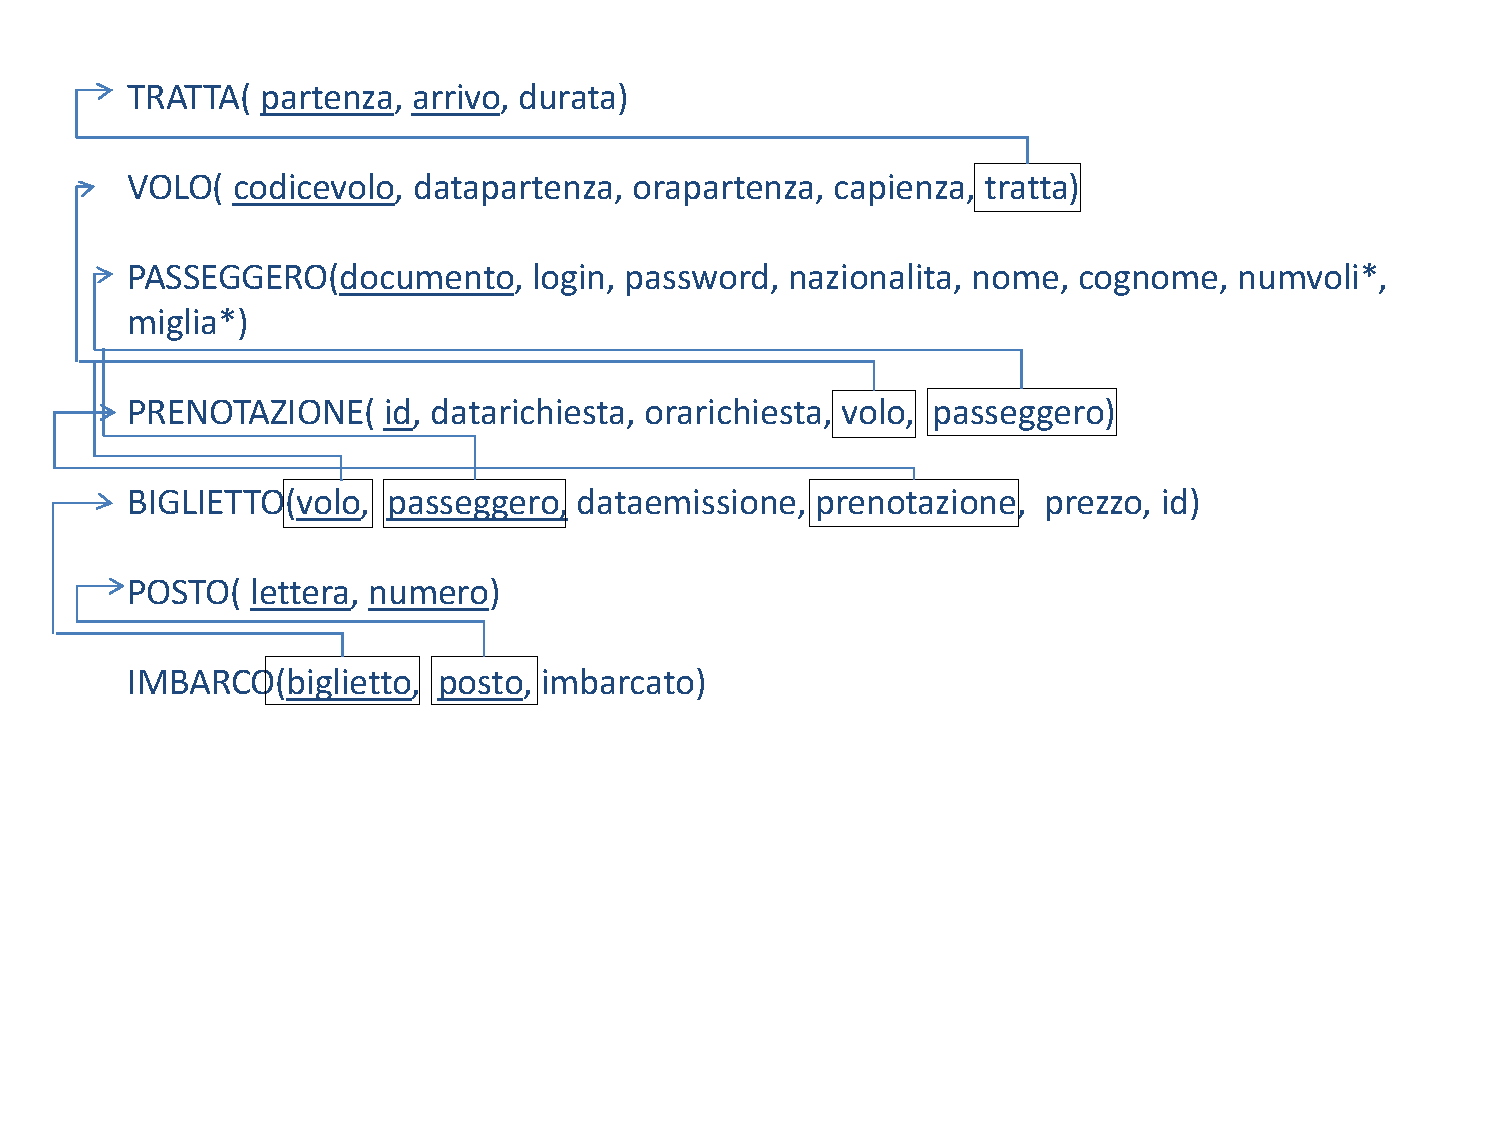
\includegraphics[scale=0.6]{schemalogico.pdf}

Descrivere il diagramma e lo schema logico.

\section{Progetto logico}

Abbiamo usato un singolo script per la creazione delle tabelle sul database. Il codice viene riportato qui di seguito.

\lstinputlisting[language=SQL, firstline=1, lastline=99]{../src/script-sql/init.sql}

Abbiamo aggiunto delle funzioni scritte in \textit{plpgsql} per eseguire azioni di routine sul base di dati e per inserire automaticamente la data e l'ora di inserimento di determinate tuple.
Si riporta di seguito il codice delle funzioni create.

\lstinputlisting[language=SQL, firstline=100, lastline=150]{../src/script-sql/init.sql}

Per automatizzare l'esecuzione delle funzioni si sono scritti dei trigger, azioni eseguite al verificarsi di certe condizioni. I trigger creati sono i seguenti:

\lstinputlisting[language=SQL, firstline=152, lastline=162]{../src/script-sql/init.sql}

 \section{Popolamento della base di dati}
 Per il popolamento della base di dati sono stati scritti dei programmi per la generazione automatica di query.
 In particolare sono stati creati dei programmi in Java per popolare le tabelle \textit{Passeggero}, \textit{Tratta} e \textit{Volo} , in grado di gestire 
 le chiavi esportate per ciascuna delle precendenti tabelle. I files .sql prodotti sono pronti 
 per essere eseguiti senza alcuna necessit\`a di modificare i files. I files per il popolamento si trovato nella cartella \textit{script\-sql} e sono \textit{popola\_tratta.sql},
 \textit{popola\_volo.sql}, \textit{popola\_passeggero}, \textit{popola\_prenotazione.sql} e \textit{popola\_biglietto.sql}.


 \newpage
\part{Progetto del sito web}

\section{Progettazione logica}

Si riportano di seguiti gli schemi di pagina seguiti durante la creazione del sito.
 \lstinputlisting[language=SQL]{page-schema/index.txt}
 \lstinputlisting[language=SQL]{page-schema/bigliettiPage.txt}
 \lstinputlisting[language=SQL]{page-schema/voliPage.txt}
 \lstinputlisting[language=SQL]{page-schema/prenotazioniPage.txt}
 \lstinputlisting[language=SQL]{page-schema/emettiBigliettoPage.txt}
 \lstinputlisting[language=SQL]{page-schema/ricercaVolo.txt}
 \lstinputlisting[language=SQL]{page-schema/login.txt}
 
\section{Struttura dell'applicazione web}

\paragraph{Architettura MVC2}
L'elaborato \`e stato sviluppato seguendo il design pattern MVC2 e seguendo l'approccio servlet-centric. Questo pattern \`e composto da tre moduli:

\begin{itemize}
 \item MODEL -  Comprende la classe DBMS.java e i Java Data Beans. I beans sono contenuti nel package \textit{bean}, mentre la classe DBMS.java \`e contenuta nel 
		package \textit{database}. DBMS.java si occupa di interrogare il DB e di manipolare i dati al suo interno. 
		La comunicazione con main.java e picture.java  avviene tramite i 
		Java Data Beans in ambo le direzioni ;
 \item VIEW - Comprende tutte le JSPs, i javascript, i css e le foto profilo salvate all'interno della base di dati;
 \item CONTROLLER - Comprende le classi \textit{main.java}, \textit{picture.java}. Entrambe sono servlet con compiti differenti: \textit{picture.java} gestisce le richieste di upload e download delle
		    immagini, \textit{main.java} controlla il flusso e gestisce il resto delle rihieste \textbf{GET} e \textbf{POST}. Utilizza \textit{DBMS}.java per l'iterazione con la base di dati ed inoltre 
		    gli eventuali dati alla JSP appropriata ;
\end{itemize}

La servlet \textit{picture.java} gestisce la parte multimediale dell'applicazione, caricando e scaricando dalla base di dati le foto profilo dei passeggeri.
La servlet identifica e gestisce le richieste HTTP sulla base che esse siano \textbf{GET} o \textbf{POST} e dal valore del parametro \textbf{ps} passato nella richiesta.

Per le richieste di tipo \textbf{GET}, \textbf{ps} pu\`o assumere questi valori:
\begin{itemize}
 \item \textbf{downloadimage} - Scrive direttamente sullo stream output l'immagine relativa al passeggero specificato.
 			     I parametri richiesti sono:
			     \begin{itemize}
			      \item \textbf{documento} Il documento del passeggero per il quale bisogna caricare l'immagine
			     \end{itemize}
 \item \textbf{Parametro assente o stringa vuota} - Viene passato il controllo a \textit{index.jsp}
\end{itemize}
Per le richieste di tipo \textbf{POST}, \textbf{ps} pu\`o assumere questi valori:
\begin{itemize}
 \item \textbf{uploadimage} - Recupera i dati del passeggero loggato e carica l'immagine passata nella base di dati. In caso di errore passa il controllo a \textit{error.jsp} specificando un messagio
			     di errore, altrimenti passa il controllo a \textit{bigliettiPage.jsp} dopo aver caricato i relativi dati.
			     I parametri richiesti sono:
			     \begin{itemize}
			      \item \textbf{image} L'immagine da caricare come foto profilo
			     \end{itemize}

 \item \textbf{Parametro assente o stringa vuota} - Viene passato il controllo a \textit{index.jsp}
\end{itemize}


La servlet \textit{main.java} controlla le richieste da parte delle JSPs.
La servlet identifica e gestisce le richieste HTTP sulla base che esse siano \textbf{GET} o \textbf{POST} e dal valore del parametro \textbf{ps} passato nella richiesta.

Per le richieste di tipo \textbf{GET}, \textbf{ps} pu\`o assumere questi valori:

\begin{itemize}
 \item \textbf{areapersonale} - Vengono caricati dalla base di dati i voli e le prenotazioni dell'utente specificato nel parametro \textit{pass}. Viene passato il controllo 
			a \textit{areapersonale.jsp}. Non sono richiesti ulteriori parametri in quanto i dati del passeggero vengono recuperati dall'attributo di sessione
			\textit{pass}.

 \item \textbf{ricercavolo} - Vengono caricati gli aeroporti di partenza e viene passato il controllo a \textit{ricercavolo.jsp}.


 \item \textbf{prenotazione} - Recupera le informazioni del volo e del passeggero. Infine passa il controllo a \textit{prenotazionePage.jsp}. 
				I parametri richiesti sono:
				\begin{itemize}
				 \item \textbf{codiceVolo} Codice del volo per recuperare le informazioni
				\end{itemize}
				
				Non serve specificare un parametro per il passeggero in quanto le informazioni vengo recuperate dall'attributo della sessione.



 \item \textbf{logout} - Viene rimosso il passeggero loggato e passa il controllo a \textit{ricercavolo.jsp} insieme agli aeroporti di partenza.


 \item \textbf{contatti} - Viene passato il controllo a \textit{contatti.jsp}
 \item \textbf{emettibiglietto} - Passa il numero della prenotazionen a \textit{emettiBigliettoPage.jsp} e gli passa il controllo. 
				  I parametri richiesti sono:
				   \begin{itemize}
				    \item \textbf{numPrenotazione} Numero della prenotazione per la quale emettere il biglietto
				   \end{itemize}


 \item \textbf{chisiamo} - Passa il controllo a \textit{chisiamo.jsp}
 \item \textbf{Parametro assente o stringa vuota} - Viene passato il controllo a \textit{index.jsp}
 \end{itemize}
 
 Per le richieste di tipo \textbf{POST}, \textbf{ps} pu\`o assumere questi valori:
 
 \begin{itemize}
 \item \textbf{newbiglietto} - Viene richiesto di emettere un biglietto a partire dal numero della prenotazione. Una volta inserito il biglietto passa il controllo a \textit{bigliettiPage.jsp} con
				i dati relativi al passeggero loggato, alle sue prenotazioni e ai suoi biglietti.
 				  I parametri richiesti sono:
				   \begin{itemize}
				    \item \textbf{numPrenotazione} Numero della prenotazione per la quale emettere il biglietto
				   \end{itemize}
 \item \textbf{login} - Vengono ricevuti la coppia login e password dalla form \textit{authentication} di \textit{login.jsp}. Se la coppia \`e valida allora passa il controllo
			 a \textit{bigliettiPage.jsp} insieme ai dati del passeggero, delle prenotazioni e dei voli. Altrimenti imposta un messaggio di errore e passa il controllo
			 a \textit{login.jsp}
			 I parametri richiesti sono:
			 \begin{itemize}
			  \item \textbf{username} Username del passeggero
			  \item \textbf{password} Password del passeggero
			 \end{itemize}
 \item \textbf{nuovaprenotazione} - Vengono inviati i dati dalla form \textit{prenotazione} di \textit{prenotazionePage.jsp}, se i dati sono validi allora si procede 
				     ad aggiungere una nuova prenotazione del database. Se il passeggero non esiste ed \`e la prima volta che effettua una prenotazione
				     allora sar\`a creato un nuovo passeggero a partire dai dati passati alla servlet. Il controllo poi passa a \textit{esitoPage.jsp} con 
				     il relativo messaggio di stato.
				     I parametri richiesti sono:
				     \begin{itemize}
				      \item \textbf{nome} Nome del passeggero
				      \item \textbf{cognome} Cognome del passeggero
				      \item \textbf{documento} Numero del documento, pu\`o essere sia il numero di una carta d'identit\`a sia di un passaporto
				      \item \textbf{nazionalita} Nazionalit\`a del passeggero
				      \item \textbf{username} Username scelto dal passeggero
				      \item \textbf{password} Password scelta dal passeggero
				      \item \textbf{codicevolo} Codice del volo da prenotare
				      \item \textbf{tessera} Richiesta della tessera
				     \end{itemize}
 \item \textbf{volipage} - Ricerca un volo a partire dai valori specificati nei parametri passati e passa il controllo a \textit{voliPage.jsp} se esiste almeno una corrispondeza, altrimenti
		  viene passato il controllo a \textit{ricercavolo.jsp}.
		  I parametri richiesti sono:
		  \begin{itemize}
		   \item \textbf{partenza} Aeroporto di partenza
		   \item \textbf{arrivo} Aeroporto di arrivo
		   \item \textbf{date} Data di partenza del volo
		  \end{itemize}
\item \textbf{Parametro assente o stringa vuota} - Viene passato il controllo a \textit{index.jsp}
 \end{itemize}


 
 
 La servlet \textit{main.java} \`e in grado di gestire anche richieste AJAX sempre con lo stesso parametro \textbf{ps}. Il parametro pu\`o assumere i seguenti valori:
 \begin{itemize}
 \item \textbf{ajaxricercavolo} - Data un aeroporto di partenza passato come parametro, ricava tutti i possibili aeroporti di arrivo. Dopo aver recuperato le informazioni invia un messaggio JSON alla JSP
				  chiamante.
				  I parametri da passare sono:
				  \begin{itemize}
				   \item \textbf{part} Indica l'aeroporto di partenza
				  \end{itemize}

 \item \textbf{checkusername} - Dato il nome utente di un passeggero interroga la classe \textit{DBMS.java} se l'username esiste all'interno della base di dati. Se esiste setta il campo \textbf{isFree} all'interno 
				del messaggio JSON di risposta a \textbf{false}, altrimenti a \textbf{true}.
				  I parametri da passare sono:
				  \begin{itemize}
				   \item \textbf{username} Indica il nome utente da controllare
				  \end{itemize}
 \item \textbf{checkdocumento} - Dato il numero di documento interroga la classe \textit{DBMS.java} se il numero di documento esiste all'interno della base di dati.
				Se esiste setta il campo \textbf{isFree} all'interno 
				del messaggio JSON di risposta a \textbf{false}, altrimenti a \textbf{true}.
 				  I parametri da passare sono:
				  \begin{itemize}
				   \item \textbf{documento} Indica il documento da controllare
				  \end{itemize}
\end{itemize}

\paragraph{Gestione di errori}
Se si verifica un errore su una qualunque pagina JSP, allora viene caricata, automaticamente dal 
sistema, la pagina \textit{error.jsp}. La pagina riporta la natura dell'errore. Se viene passato il parametro \textbf{msg} allora 
stamper\`a il messaggio di errore specificato.

\paragraph{Pagine JSPs e parametri passati}

Vengono descritte ora le JSPs utilizzate con i relativi parametri.

\begin{itemize}
 \item \textit{index.jsp} - Home page del sito. Viene mostrato un men\`u con il quale \`e possibile muoversi. La pagina \`e composta da un iframe a cui interno vengono
			    caricate le singole JSPs. 
			    
 \item \textit{error.jsp} - Se si verifica un errore su una qualunque pagina JSP, allora viene caricata, automaticamente dal 
			    sistema, la pagina \textit{error.jsp}. La pagina riporta la natura dell'errore. Se viene passato il parametro \textbf{msg} allora 
			    stamper\`a il messaggio di errore specificato. 
 			Parametri passati alla pagina:
			\begin{itemize}
			 \item \textbf{msg} Messaggio di errore da stampare
			\end{itemize}
			
 \item \textit{bigliettiPage.jsp} - Pagina personale del passeggero dove vengono mostrati i dati personali, i biglietti e le prenotazioni. \`E possibile emettere un biglietto cliccando sul link del codice 
				    del volo nella tabella inerente alle prenotazioni. Il codice \`e un link per la pagina \textit{emettiBigliettoPage.jsp}. \`E presente una form per caricare
				    un'immagine personale come immagine profilo. Se non \`e specificata un'immagine all'interno della base di dati allora la JSP caricher\`a un'immagine di default.
 			Parametri passati alla pagina:
			\begin{itemize}
			 \item \textbf{prenotazioni} Tutte le prenotazioni del passeggero che si \`e logggato
			 \item \textbf{biglietti} Tutti i biglietti emessi del passeggero loggato
			 \item \textbf{pass} Oggetto di tipo PasseggeroBean con le informazioni del passeggero
			\end{itemize}
			
 \item \textit{chisiamo.jsp} - Pagina riportante una breve descrizione della societ\`a e del loro operato;
 
 \item \textit{contatti.jsp} - Pagina dove si possono trovare i contatti dell'azienda, con un form per inviare una mail;
 
 \item \textit{emettiBigliettoPage.jsp} - Pagina dove si emette il biglietto a partire da una prenotazione. 
 			Parametri passati alla pagina:
			\begin{itemize}
			 \item \textbf{numPrenotazione} Numero della prenotazione per la quale si vuole immettere il biglietto.
			\end{itemize}
			
 \item \textit{esitoPage.jsp} - Pagina di esito per la prenotazione. Se la prenotazione \`e andata a buon fine verr\`a visualizzato un messaggio di conferma,
				altrimenti di errore.
 			Parametri passati alla pagina:
			\begin{itemize}
			 \item \textbf{status} Esito della prenotazione.
			\end{itemize}
			
 \item \textit{login.jsp} - Pagina per il login del passeggero. Prima di effettuare il login il passeggero deve aver prenotato almeno un volo.
			Parametri passati alla pagina:
			\begin{itemize}
			 \item \textbf{auth} Messaggio di errore se l'autenticazione precedente non \`e andata a buon fine
			\end{itemize}
			
 \item \textit{prenotazionePage.jsp} - Pagina dove vengono mostrati i dettagli del volo scelto ed una form per la prenotazione del volo.
				      I dati inseriti nella form vengono controllati da una funzione JQUERY. Ogni campo ha collegato una funzione per la verifica della correttezza
				      dei dati inseriti. I campi \textbf{documento} e \textbf{username} vengono validati real-time tramite due funzioni AJAX, una per validare il documento e l'altra per l'username.
				      Entrambe le funzioni richiedono una conferma alla servlet sulla disponibilit\`a del nome utente e del documento. Per entrambi si controlla che non esistano gi\`a all'interno
				      della base di dati. Per gli altri campi viene eseguito un controllo sulla lunghezza e sul contenuto.
 			Parametri passati alla pagina:
			\begin{itemize}
			 \item \textbf{volo} Oggetto di tipo VoloBean con all'interno tutte le informazioni sul volo scelto
			 \item \textbf{pass} Oggetto di tipo PasseggeroBean con le informazioni del passeggero. Questo parametro \`e diverso da \textit{null} 
				solo se il passeggero ha effettuato il login in precedenza.
			\end{itemize}
			
 \item \textit{ricercavolo.jsp} - Pagina per la ricerca di un volo. Mediante la form si devono scegliere un aeroporto di partenza, un aeroporto di arrivo e la data 
				 di partenza. 
				 Gli aeroporti di arrivo vengono caricati in un secondo momento, appena l'utente sceglie l'aeroporto di partenza, una funzione AJAX richiede alla servlet tutti gli
				 aeroporti collegati all'aeroporto di partenza scelto.
				 Il campo per la scelta della data di partenza presenta un ``datepicker'' di default che si disabilita quando riconosce come browser ``Chrome''. Questo perch\'e 
				 ``Chrome'' ha gi\`a incorporato un datepicker quando rileva, all'interno di una form, un campo di type \textit{date}.
 			Parametri passati alla pagina:
			\begin{itemize}
			 \item \textbf{partenze} Sono tutti gli aeroporti dai quali \`e possibile partire
			 \item \textbf{status} Messaggio usato se non vengono trovati dei voli a partire dai criteri scelti.
			\end{itemize}
			
 \item \textit{voliPage.jsp} - Pagina dove vengono mostrati i voli trovati dopo la selezione attraverso la form di \textit{ricercavolo.jsp}. Il codice \`e un link per la pagina \textit{prenotazionePage.jsp}.
 			Parametri passati alla pagina:
			\begin{itemize}
			\item \textbf{voli} ArrayList dei voli richiesti 
			\end{itemize}
\end{itemize}

\paragraph{Path e Context}
Il context del sito web \`e \textit{basi}, mentre il path relativo per raggiungere la servlet \`e \textit{servlet/main}. La porta del server \`e la \textit{8080}.
Quindi l'url per accedere al sito web \`e: \url{http://localhost:8080/basi/servlet/main}

\paragraph{Login e sessioni}
Quando un passeggero esegue il login viene associata una sessione al client relativo, nella quale viene mantenuto
l'attributo \textbf{pass}. L'attributo contiene l'oggetto relativo al passeggero loggato.
L'utilizzo di sessioni implica che il browser del client debba avere l'accettazione 
di COOKIE attiva per poter navigare sul sito.
Ogni sessione dura 600 secondi(10 minuti), dopo di che  essa verr\`a ``eliminata'' e se 
avviene   un   altra   richiesta   da   parte   di   un   host   a   cui   \`e   scaduta   la   sessione,   allora   esso   verr\`a 
reindirizzato alla \textit{index.jsp}.

\part{Scelte progettuali}
  
 \section{Ipotesi e strategie adotattate}
  \begin{itemize}
   \item La relazione \textit{passeggero} ha \textbf{documento} e\textbf{login} come possibili identificatori. \`E stato scelto di usare il documento come chiave primaria, mantenendo comuqnue
   l'attributo login univoco sulla tabella.
   \item Per la relazione \textit{biglietto} non \`e stato utilizzato l'identificatore univoco come chiave primaria per poter avere una consistenza nella base di dati.
   \item L'attributo \textbf{data\_emissione} nell'entit\`a \textit{biglietto} viene aggiunto automaticamente da una funzione trigger, spiegata nella relazione.
   \item Gli attributi \textbf{data\_richiesta} e \textbf{ora\_richiesta} nell'entit\`a \textit{prenotazione} viene aggiunto automaticamente da una funzione trigger, spiegata nella relazione.
   \item Si \`e aggiunto l'attributo \textbf{imbarcato} nella relazione \textit{imbarco} in quanto il biglietto viene sempre assegnato ad un posto, per\`o il passeggero pu\`o non imbarcarsi sull'aereo.
   \item All'interno delle servlet sono state utilizzate le classi Command per la gestione delle azioni da intraprendere quando si riceve una richiesta. Tutte le classe estendo un'interfaccia comune di nome \textit{Command.java}.
  \end{itemize} 


 \section{Hibernate}
 Hibernate \`e una piattaforma middleware open source per lo sviluppo di applicazioni Java, 
 attraverso l'appoggio al relativo framework, che fornisce un servizio di Object-relational mapping (ORM) ovvero gestisce la persistenza dei dati 
 sul database attraverso la rappresentazione e il mantenimento su database relazionale di un sistema di oggetti Java.
 
 Per la creazione dei Java Data Beans si \`e utilizzato un plugin di Eclipse di nome JBoss Tools. Questo pacchetto permette di creare i Java Data Beans relativi alle tabelle all'interno di un database.
 
 \section{AJAX}
 AJAX è una tecnica di sviluppo software per la realizzazione di applicazioni web interattive. Consiste nel creare una servlet Java che riceve parametri da parte 
 di una pagina web (nel nostro caso una JSP); questa servlet elabora i dati e li invia alla pagina chiamante, 
 in modo che possa ricevere dinamicamente dati e quindi modificare il suo aspetto o comportamento.
 
 Si è voluta utilizzare questa tecnologia per rendere dinamica la selezione in un campo del form di tipo select; 
 poiché però questi campi devono essere ``popolati'' con dati provenienti dal database, è stato necessario introdurre la tecnologia JQuery e JSON.
 
 JQuery consiste in un insieme di librerie per semplificare la programmazione web, nel nostro caso è stato utilizzato internamente ad 
 AJAX per eseguire una query sul database e mappare in un LinkedHashMap la risposta. Per inviare poi questa risposta alla pagina web, è stato utilizzato JSON, 
 una teconogia che consente lo scambio di dati tra architetture client-server;

\end{document}          
